w\chapter{IMPLEMENTASI}
  Pada bab ini dibahas mengenai implementasi aplikasi sesuai dengan perancangan sistem yang telah dijelaskan sebelumnya. Bahasa pemrograman yang digunakan antara lain PHP, SQL, Javascript.
  
  \section{Lingkungan Implementasi}
  Lingkungan pembangunan dijelaskan pada subbab ini.
  \subsection{Lingkungan Pembangun Perangkat Keras}
  Perangkat keras yang digunakan dalam pembuatan tugas akhir ini adalah sebagai berikut :
  \begin{enumerate}
  \item Personal Komputer
  		\begin{enumerate}
  		\item Prosesor XX
        \item Memori YY
        \item Sistem Operasi ZZ
  		\end{enumerate}
  \item VPS
  	VPS yang digunakan dalam lingkungan pembangunan di\textit{host} oleh DigitalOcean dengan spesifikasi sebagai berikut :
  		\begin{enumerate}
  		\item Prosesor XX
        \item Memori YY
        \item Sistem Operasi ZZ
  		\end{enumerate}
  \end{enumerate}
  
  \subsection{Lingkungan Pembangun Perangkat Lunak}
  Spesifikasi perangkat lunak yang digunakan untuk membuat tugas akhir ini adalah sebagai berikut:
  \begin{enumerate}
  \item Web Browser Google Chrome
  \item PgAdmin
  \item PHPStorm sebagai IDE PHP
  \item Nano untuk \textit{shell text editor}
  \item Postman
  \item Power Designer
  \end{enumerate}
  
\section{Implementasi Antarmuka}
	
    \subsection{Antarmuka Halaman A}
    Penjelasan otorisasi terhadap antarmuka A, link yang tersedia dalam antarmuka A, dan penjelasan \textit{exception} jika terjadi masalah baik otorisasi ataupun autentikasi saat mengakses antarmuka ini.
  
      \begin{figure}[H]
        \centering
        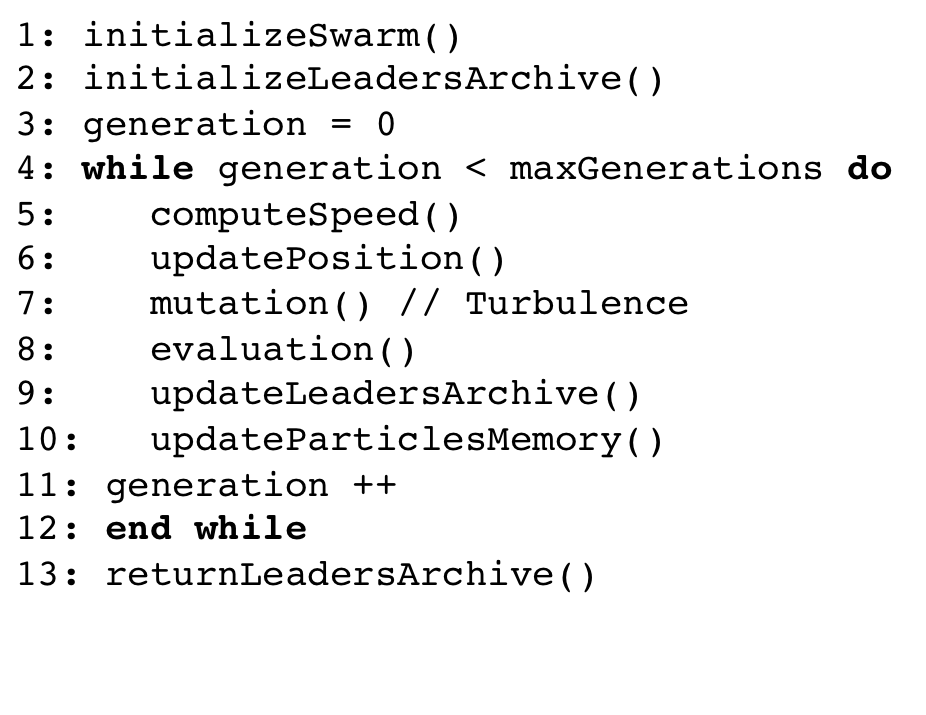
\includegraphics[width=\linewidth]{images/bab4/smpso_code.png}
        \caption{ Pseudocode Controller untuk Menampilkan Antarmuka A }
        \label{pdm}
      \end{figure}
      
    \subsection{Antarmuka Halaman B}
    Penjelasan otorisasi terhadap antarmuka B, link yang tersedia dalam antarmuka B, dan penjelasan \textit{exception} jika terjadi masalah baik otorisasi ataupun autentikasi saat mengakses antarmuka ini.
  
      \begin{figure}[H]
        \centering
        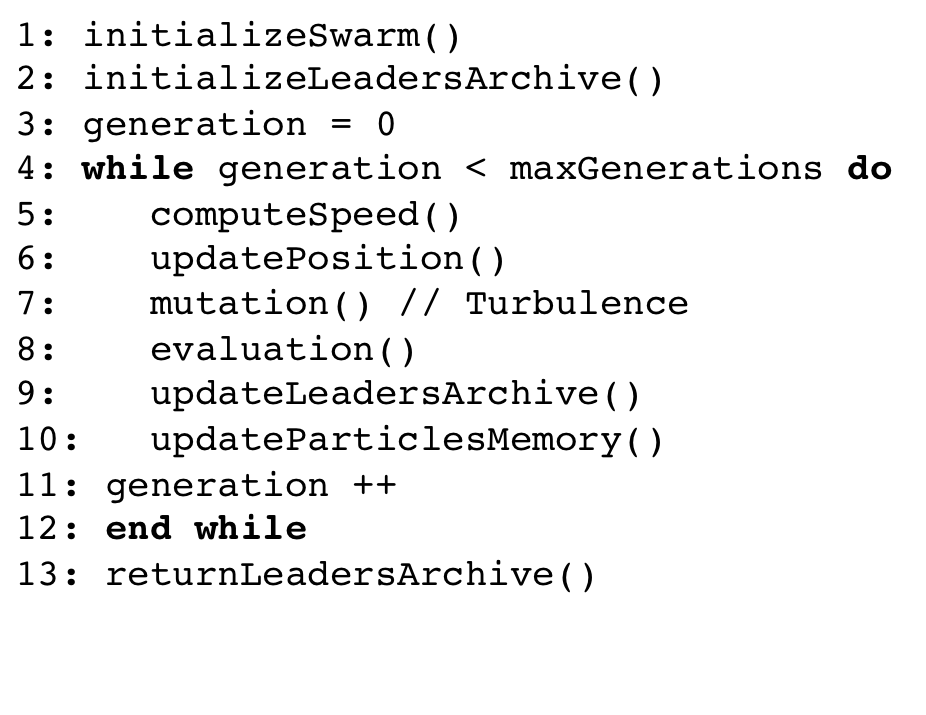
\includegraphics[width=\linewidth]{images/bab4/smpso_code.png}
        \caption{ Pseudocode Controller untuk Menampilkan Antarmuka B }
        \label{pdm}
      \end{figure}
    
    
\section{Pemasangan Proyek}
	Pembangunan dilakukan secara online, dan tersebar (tidak hanya menggunakan satu \textit{service provider} saja.
    Berikut dijelaskan langkah-langkah pembangunan proyek:
    
    \subsection{Konfigurasi Domain}
    Domain yang dipilih berasal dari Namecheap.com , dengan langkah-langkah konfigurasi sebagai berikut :
    \begin{enumerate}
    \item Langkah 1
    \item Langkah 2
    \end{enumerate}
    \subsection{Konfigurasi VPS}
    Domain yang dipilih berasal dari DigitalOcean dan Google Cloud Computing , dengan langkah-langkah konfigurasi sebagai berikut :
    \begin{enumerate}
    \item DigitalOcean
      \begin{enumerate}
      \item Langkah 1
      \item Langkah 2
      \end{enumerate}
    \item Google Cloud Computing
      \begin{enumerate}
      \item Langkah 1
      \item Langkah 2
      \end{enumerate}
    \end{enumerate}
    
    \subsection{Konfigurasi PostgreSQL}
    PostgreSQL diinstal dalam VPS, dengan langkah-langkah konfigurasi sebagai berikut :
    \begin{enumerate}
    \item Langkah 1
    \item Langkah 2
    \end{enumerate}
    
    \subsection{Konfigurasi Node.js}
    Node.js diinstall dalam VPS, dengan langkah-langkah konfigurasi sebagai berikut :
    \begin{enumerate}
    \item Langkah 1
    \item Langkah 2
    \end{enumerate}
    
    \subsection{Konfigurasi MongoDB}
    MongoDB diinstall dalam VPS, dengan langkah-langkah konfigurasi sebagai berikut :
    \begin{enumerate}
    \item Langkah 1
    \item Langkah 2
    \end{enumerate}
    
    \subsection{Konfigurasi SMTP Service}
    SMTP \textit{service} yang digunakan berasal dari sendgrid.net, dengan langkah-langkah konfigurasi sebagai berikut :
    \begin{enumerate}
    \item Langkah 1
    \item Langkah 2
    \end{enumerate}
